\chapter{راهنمای استفاده از الگوی لاتک دانشگاه صنعتی امیرکبیر(پلی‌تکنیک تهران)}

\section{مقدمه}
حروف‌چینی پروژه کارشناسی، پایان‌نامه یا رساله یکی از موارد پرکاربرد استفاده از زی‌پرشین است. از طرفی، یک پروژه، پایان‌نامه یا رساله،  احتیاج به تنظیمات زیادی از نظر صفحه‌آرایی  دارد که ممکن است برای
یک کاربر مبتدی، مشکل باشد. به همین خاطر، برای راحتی کار کاربر، یک کلاس با نام 
\verb;AUTthesis;
 برای حروف‌چینی پروژه‌ها، پایان‌نامه‌ها و رساله‌های دانشگاه صنعتی امیرکبیر با استفاده از نرم‌افزار زی‌پرشین،  آماده شده است. این فایل به 
گونه‌ای طراحی شده است که کلیه خواسته‌های مورد نیاز  مدیریت تحصیلات تکمیلی دانشگاه صنعتی امیرکبیر را برآورده می‌کند و نیز، حروف‌چینی بسیاری
از قسمت‌های آن، به طور خودکار انجام می‌شود.

کلیه فایل‌های لازم برای حروف‌چینی با کلاس گفته شده، داخل پوشه‌ای به نام
\verb;AUTthesis;
  قرار داده شده است. توجه داشته باشید که برای استفاده از این کلاس باید فونت‌های
  \verb;Nazanin B;،
 \verb;PGaramond;
 (اینو نداریم فعلا)
 و
  \verb;IranNastaliq;
    روی سیستم شما نصب شده باشد.
\section{این همه فایل؟!}\label{sec2}
از آنجایی که یک پایان‌نامه یا رساله، یک نوشته بلند محسوب می‌شود، لذا اگر همه تنظیمات و مطالب پایان‌نامه را داخل یک فایل قرار بدهیم، باعث شلوغی
و سردرگمی می‌شود. به همین خاطر، قسمت‌های مختلف پایان‌نامه یا رساله  داخل فایل‌های جداگانه قرار گرفته است. مثلاً تنظیمات پایه‌ای کلاس، داخل فایل
\verb;AUTthesis.cls;، 
تنظیمات قابل تغییر توسط کاربر، داخل 
\verb;commands.tex;،
قسمت مشخصات فارسی پایان‌نامه، داخل 
\verb;fa_title.tex;,
مطالب فصل اول، داخل 
\verb;chapter1;
و ... قرار داده شده است. نکته مهمی که در اینجا وجود دارد این است که از بین این  فایل‌ها، فقط فایل 
\verb;AUTthesis.tex;
قابل اجرا است. یعنی بعد از تغییر فایل‌های دیگر، برای دیدن نتیجه تغییرات، باید این فایل را اجرا کرد. بقیه فایل‌ها به این فایل، کمک می‌کنند تا بتوانیم خروجی کار را ببینیم. اگر به فایل 
\verb;AUTthesis.tex;
دقت کنید، متوجه می‌شوید که قسمت‌های مختلف پایان‌نامه، توسط دستورهایی مانند 
\verb;input;
و
\verb;include;
به فایل اصلی، یعنی 
\verb;AUTthesis.tex;
معرفی شده‌اند. بنابراین، فایلی که همیشه با آن سروکار داریم، فایل 
\verb;AUTthesis.tex;
است.
در این فایل، فرض شده است که پایان‌نامه یا رساله شما، از5 فصل و یک پیوست، تشکیل شده است. با این حال، اگر
  پایان‌نامه یا رساله شما، بیشتر از 5 فصل و یک پیوست است، باید خودتان فصل‌های بیشتر را به این فایل، اضافه کنید. این کار، بسیار ساده است. فرض کنید بخواهید یک فصل دیگر هم به پایان‌نامه، اضافه کنید. برای این کار، کافی است یک فایل با نام 
\verb;chapter6;
و با پسوند 
\verb;.tex;
بسازید و آن را داخل پوشه 
\verb;AUTthesis;
قرار دهید و سپس این فایل را با دستور 
\texttt{\textbackslash include\{chapter6\}}
داخل فایل
\verb;AUTthesis.tex;
و بعد از دستور
\texttt{\textbackslash include\{chapter6\}}
 قرار دهید.

\section{از کجا شروع کنم؟}
قبل از هر چیز، بدیهی است که باید یک توزیع تِک مناسب مانند 
\verb;Live TeX;
و یک ویرایش‌گر تِک مانند
\verb;Texmaker;
را روی سیستم خود نصب کنید.  نسخه بهینه شده 
\verb;Texmaker;
را می‌توانید  از سایت 
 \href{http://www.parsilatex.com}{پارسی‌لاتک}%
\LTRfootnote{\url{http://www.parsilatex.com}}
 و
\verb;Live TeX;
را هم می‌توانید از 
 \href{http://www.tug.org/texlive}{سایت رسمی آن}%
\LTRfootnote{\url{http://www.tug.org/texlive}}
 دانلود کنید.
 
در مرحله بعد، سعی کنید که  یک پشتیبان از پوشه 
\verb;AUTthesis;
 بگیرید و آن را در یک جایی از هارددیسک سیستم خود ذخیره کنید تا در صورت خراب کردن فایل‌هایی که در حال حاضر، با آن‌ها کار می‌کنید، همه چیز را از 
 دست ندهید.
 
 حال اگر نوشتن پایان‌نامه اولین تجربه شما از کار با لاتک است، توصیه می‌شود که یک‌بار به طور سرسری، کتاب «%
\href{http://www.tug.ctan.org/tex-archive/info/lshort/persian/lshort.pdf}{مقدمه‌ای نه چندان کوتاه بر
\lr{\LaTeXe}}\LTRfootnote{\url{http://www.tug.ctan.org/tex-archive/info/lshort/persian/lshort.pdf}}»
   ترجمه دکتر مهدی امیدعلی، عضو هیات علمی دانشگاه شاهد را مطالعه کنید. این کتاب، کتاب بسیار کاملی است که خیلی از نیازهای شما در ارتباط با حروف‌چینی را برطرف می‌کند.
 
 
بعد از موارد گفته شده، فایل 
\verb;AUTthesis.tex;
و
\verb;fa_title;
را باز کنید و مشخصات پایان‌نامه خود مثل نام، نام خانوادگی، عنوان پایان‌نامه و ... را جایگزین مشخصات موجود در فایل
\verb;fa_title;
 کنید. دقت داشته باشید که نیازی نیست 
نگران چینش این مشخصات در فایل پی‌دی‌اف خروجی باشید. فایل 
\verb;AUTthesis.cls;
همه این کارها را به طور خودکار برای شما انجام می‌دهد. در ضمن، موقع تغییر دادن دستورهای داخل فایل
\verb;fa_title;
 کاملاً دقت کنید. این دستورها، خیلی حساس هستند و ممکن است با یک تغییر کوچک، موقع اجرا، خطا بگیرید. برای دیدن خروجی کار، فایل 
\verb;fa_title;
 را 
\verb;Save;، 
(نه 
\verb;As Save;)
کنید و بعد به فایل 
\verb;AUTthesis.tex;
برگشته و آن را اجرا کنید. حال اگر می‌خواهید مشخصات انگلیسی پایان‌نامه را هم عوض کنید، فایل 
\verb;en_title;
را باز کنید و مشخصات داخل آن را تغییر دهید.%
\RTLfootnote{
برای نوشتن پروژه کارشناسی، نیازی به وارد کردن مشخصات انگلیسی پروژه نیست. بنابراین، این مشخصات، به طور خودکار،
نادیده گرفته می‌شود.
}
 در اینجا هم برای دیدن خروجی، باید این فایل را 
\verb;Save;
کرده و بعد به فایل 
\verb;AUTthesis.tex;
برگشته و آن را اجرا کرد.

برای راحتی بیشتر، 
فایل 
\verb;AUTthesis.cls;
طوری طراحی شده است که کافی است فقط  یک‌بار مشخصات پایان‌نامه  را وارد کنید. هر جای دیگر که لازم به درج این مشخصات باشد، این مشخصات به طور خودکار درج می‌شود. با این حال، اگر مایل بودید، می‌توانید تنظیمات موجود را تغییر دهید. توجه داشته باشید که اگر کاربر مبتدی هستید و یا با ساختار فایل‌های  
\verb;cls;
 آشنایی ندارید، به هیچ وجه به این فایل، یعنی فایل 
\verb;AUTthesis.cls;
دست نزنید.

نکته دیگری که باید به آن توجه کنید این است که در فایل 
\verb;AUTthesis.cls;،
سه گزینه به نام‌های
\verb;bsc;,
\verb;msc;
و
\verb;phd;
برای تایپ پروژه، پایان‌نامه و رساله،
طراحی شده است. بنابراین اگر قصد تایپ پروژه کارشناسی، پایان‌نامه یا رساله را دارید، 
 در فایل 
\verb;AUTthesis.tex;
باید به ترتیب از گزینه‌های
\verb;bsc;،
\verb;msc;
و
\verb;phd;
استفاده کنید. با انتخاب هر کدام از این گزینه‌ها، تنظیمات مربوط به آنها به طور خودکار، اعمل می‌شود.

\section{مطالب پایان‌نامه را چطور بنویسم؟}
\subsection{نوشتن فصل‌ها}
همان‌طور که در بخش 
\ref{sec2}
گفته شد، برای جلوگیری از شلوغی و سردرگمی کاربر در هنگام حروف‌چینی، قسمت‌های مختلف پایان‌نامه از جمله فصل‌ها، در فایل‌های جداگانه‌ای قرار داده شده‌اند. 
بنابراین، اگر می‌خواهید مثلاً مطالب فصل ۱ را تایپ کنید، باید فایل‌های 
\verb;AUTthesis.tex;
و
\verb;chapter1;
را باز کنید و محتویات داخل فایل 
\verb;chapter1;
را پاک کرده و مطالب خود را تایپ کنید. توجه کنید که همان‌طور که قبلاً هم گفته شد، تنها فایل قابل اجرا، فایل 
\verb;AUTthesis.tex;
است. لذا برای دیدن حاصل (خروجی) فایل خود، باید فایل  
\verb;chapter1;
را 
\verb;Save;
کرده و سپس فایل 
\verb;AUTthesis.tex;
را اجرا کنید. یک نکته بدیهی که در اینجا وجود دارد، این است که لازم نیست که فصل‌های پایان‌نامه را به ترتیب تایپ کنید. می‌توانید ابتدا مطالب فصل ۳ را تایپ کنید و سپس مطالب فصل ۱ را تایپ کنید.

نکته بسیار مهمی که در اینجا باید گفته شود این است که سیستم
\lr{\TeX},
محتویات یک فایل تِک را به ترتیب پردازش می‌کند. به عنوان مثال، اگه فایلی، دارای ۴ خط دستور باشد، ابتدا خط ۱، بعد خط ۲، بعد خط ۳ و در آخر، خط ۴ پردازش می‌شود. بنابراین، اگر مثلاً مشغول تایپ مطالب فصل ۳ هستید، بهتر است
که دو دستور
\verb~\chapter{مقدمه}

\section{مقدمه}
در صنعت، نگهداری و تعمیرات\LTRfootnote{Maintenance} به تمام فعالیت‌هایی اطلاق می‌شود که بر روی ابزارهای صنعتی انجام می‌شود تا بهره‌وری و عمر این ابزارها افزایش یابد. در سال‌های اخیر، رویکردهای مختلفی برای انجام نگهداری مورد استفاده قرار گرفته است. روش‌های نگهداری زیر، از میان همه‌ی این رویکردها، بیشترین فراوانی استفاده در صنعت را دارند\cite{zhao2022review}:

\begin{itemize}

\item \textbf{نگهداری و تعمیرات اصلاحی\LTRfootnote{Corrective Maintenance}}: به جایگزینی قطعه خراب‌شده در سیستم می‌پردازد. در این رویکرد، تا زمانیکه فرایند جایگزینی قطعه معیوب به اتمام نرسد، سیستم غیرقابل بهره‌برداری است و تعمیر قطعات بعد از خرابی هزینه‌های قابل توجهی برای صاحبان صنعت به همراه دارد\cite{ran2019survey}.

\item \textbf{نگهداری و تعمیرات جلو‌گیرانه\LTRfootnote{Preventive Maintenance}}: سعی در پیش‌گیری از اتلاف زمان ناشی از توقف اضطراری دارد، اما در عوض ممکن است تعدادی از قطعاتی که هنوز عمر مفید دارند، دور ریخته شوند و اسراف در هزینه و قطعات مصرفی صورت گیرد\cite{ran2019survey}.

\item \textbf{نگهداری و تعمیرات پیش‌بینانه\LTRfootnote{Predictive Maintenance}}: سعی می‌کند مشکلات دو نوع نگهداری و تعمیرات مذکور را حل کند. با استفاده از این روش، زمان عملیاتی هر قسمت دستگاه تخمین زده می‌شود و قطعاتی که توسط سیستم مشکوک به خرابی در آینده هستند تعویض می‌گردند و بنابراین ابزارهای موجود در سیستم به صورت بهینه مورد استفاده قرار می‌گیرند و هزینه‌های تعمیرات بشدت کاهش می‌یابد\cite{zonta2020predictive, ran2019survey}.

\end{itemize}

بدلیل اینکه در نگهداری پیش‌بینانه قطعات در حال خرابی، پیش از وقوع خرابی شناسایی می‌شوند و ناکارآمدی آن بخش به کل سیستم آسیب نمی‌رساند، همانطور که در \cref{fig:maintenance_comparison} مشخص است، با استفاده از این نوع نگهداری، می‌توان مجموع هزینه‌های نگهداری و تعمیرات را به حداقل میزان ممکن رساند\cite{zonta2020predictive}.

\begin{figure}[!h]
\centerline{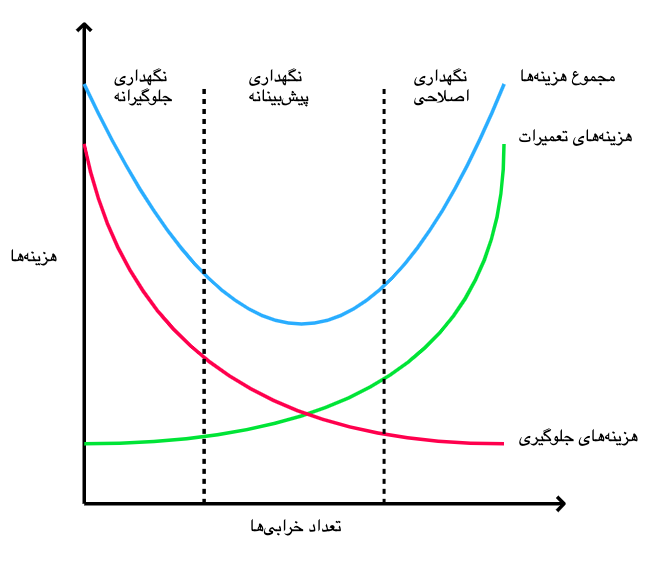
\includegraphics[width=.8\textwidth]{maintenance_comparison.png}}
\caption{مقایسه‌ی هزینه‌های انواع نگهد‌اری‌ها}
\label{fig:maintenance_comparison}
\end{figure}


\section{تعریف مسئله}
هدف از انجام این پروژه، پیاده‌سازی سیستمی برای اجراکردن نگهداری پیش‌بینانه بر روی گره‌های موجود در یک اینترنت اشیاء\LTRfootnote{Internet of Things} بهم پیوسته است. رویکردهای مختلفی برای این منظور تا کنون توسط محققان ابداع و مورد استفاده قرار گرفته شده است. از جمله‌ی این موارد می‌توان به تحلیل لرزش\LTRfootnote{Vibration Analysis} اشاره کرد. برای پیاده‌سازی این سیستم همانطور که در \cref{fig:workflow} به تصویر آمده ‌است، نیازمند آنیم که داده‌های لرزش مربوط به گره‌ها را که توسط یک سیستم قابل‌اتکا\LTRfootnote{Reliable} جمع‌آوری شده است، دریافت کرده و با جداکردن داده‌های پرت\LTRfootnote{Outlier Data}، از بین‌بردن تاثیر اختلال\LTRfootnote{Noise} ایجادشده توسط گرانش و خرابی یا درست‌ کارنکردن حسگر\LTRfootnote{Sensor} اندازه‌گیری لرزش، استخراج ویژگی‌\LTRfootnote{Feature Extraction}های مناسب برای انجام تحلیل روی داده و درنهایت پیشنهاد دادن مدلی برای نحوه‌ی یادگیری ماشین\LTRfootnote{Machine Learning} و تحلیل و مقایسه‌ی داده‌های بدست‌آمده با داده‌های برچسب‌دار\LTRfootnote{Labeled Data}، عمر باقی‌مانده\LTRfootnote{Remaining Useful Lifetime}‌ی دستگاه‌های مختلف را پیش‌بینی کنیم و بر اساس اعداد بدست‌آمده، اقدامات مناسب را برای انجام مراقبت‌های دوره‌ای انجام دهیم و از تحمیل‌شدن هزینه‌های جانبی در آینده جلوگیری کنیم\cite{jung2017vibration}. برای راحتی استفاده از سیستم طراحی‌شده، مستقرساختن\LTRfootnote{Deploy} سرویس توسعه‌یافته‌شده روی ابر\LTRfootnote{Cloud} و همچنین احراز هویّت مدیر\LTRfootnote{Admin}ان و دروازه\LTRfootnote{Gateway}‌های ارسال‌کننده داده‌ی لرزش کارگزار\LTRfootnote{Server}ی نیز پیاده خواهد شد.

\begin{figure}[!h]
\centerline{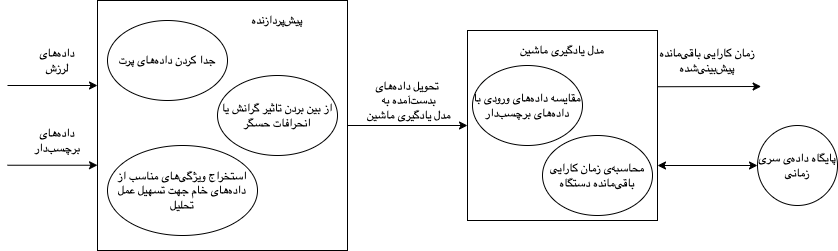
\includegraphics[width=1\textwidth]{workflow.png}}
\caption{نمودار جریان کار}
\label{fig:workflow}
\end{figure}


\section{کارهای مشابه}
نگهداری و تعمیرات پیش‌بینانه نسبتاً موضوع نو ظهوری است و عمر کمتری را نسبت به انواع دیگر نگهداری‌های موجود دارد. اما با این‌حال تا به امروز تلاش‌های قابل‌توجهی برای بکارگیری این نوع از نگهداری در سطح دنیا صورت گرفته است که در اینجا به مواردی که رویکردهای جالبی داشته‌اند اشاره خواهیم کرد. در \cite{tinga2010application} مدلی براي خرابی قطعات مبتنی بر ميزان استفاده از تجهيزات و بار داخلی آنها ارائه شده‌است اما مدل ارائه‌شده محدود به يک مدل تجهيزات است و براي استفاده در ساير مدل‌ها نظارت مجدد لازم است. در \cite{wu2007neural} روندی مبتنی بر شبكه‌های عصبی جهت پيش‌بينی عمر مفيد باقی‌مانده تجهيزات چرخشی ارائه شده‌است اما تنها مختص به اين دسته از تجهيزات است. در \cite{kaiser2009predictive} رويكردی مبتنی بر شبكه عصبی جهت پيش‌بينی زمان نگهداری و تعميرات تجهيزات بر اساس مدل خرابی و كارايی آنها ارائه می‌شود اما در یک محيط شبيه‌سازی‌شده و كنترل‌شده آزمايش شده‌است و در هنگام استفاده در محيط واقعی غيرعملی است.

 بطور كلی در پژوهش‌های يادشده روندهای در پیش‌گرفته‌شده برای پیش‌بینی خرابی و زمان آن، مختص نوع خاصی از تجهيزات است و در يک محيط آزمايشگاهی و كنترل‌شده ارزيابی شده‌اند. در حالی‌كه در اين پروژه با استفاده از داده‌های جمع‌آوری‌شده از قطعات مختلف سعی كرده‌ايم رويكردی كلی و مناسب محيط واقعی و صنعتی ارائه دهيم. همچنین شایان ذکر است که در هیچ‌کدام از پروژه‌های یاد‌شده، سیستم طراحی‌شده روی ابر مستقر نشده‌اند و سرویس‌هایی همانند احراز هویت و برنامه‌ی تحت وب برای آنها طراحی نشده است. این در حالی است که در این پروژه قصد بر این بوده که سیستمی کلی برای مدیریت بهتر قطعات با جلوه‌ای مناسب طراحی گردد و توسعه یابد.
~
و
\verb~\chapter{تکنولوژی‌های استفاده‌شده}

در این فصل تکنولوژی‌ها و چارچوب\LTRfootnote{Framework}‌های اصلی دخیل در توسعه این دستگاه را به طور دقیق مورد بررسی قرار می‌دهیم.

\section{‌‌زبان برنامه‌نویسی}
برای انتخاب زبان برنامه‌نویسی مناسب برای توسعه مدل یادگیری ماشین شرح‌داده شده، باید معیارهای متفاوتی را در نظر گرفت. برای این منظور زبان پایتون\LTRfootnote{\href{https://docs.python.org/3/}{Python}} را برگزیدیم. مواردی همچون داشتن چارچوب‌ها و کتابخانه‌های قدرتمند یادگیری ماشین، توسعه‌ی آسان و سریع و محبوبیت بالا از دلایل اصلی انتخاب پایتون به عنوان زبان اصلی برای توسعه‌ی سرویس یادگیری ماشین می‌باشد. همچنین شایان ذکر است که چون کارگزار اصلی جمع‌آوری اطلاعات لرزش به زبان پایتون نوشته شده است، استفاده از این زبان برای توسعه مدل یادگیری ماشین، باعث بهبود توسعه‌پذیری نیز می‌گردد. 

\subsection{زبان برنامه‌نویسی پایتون}
یک زبان برنامه‌نویسی عمومی و سطح بالا است که فلسفه طراحی آن بر روی خوانایی کد تأکید دارد. نحو\LTRfootnote{Syntax} پایتون به برنامه‌نویسان امکان می‌دهد تا مفاهیم را با تعداد کمتری خط کد نسبت به زبان‌هایی مانند سی\LTRfootnote{C Programming Language} بیان کنند و این زبان ساختارهایی را فراهم می‌کند که برنامه‌های واضح و قابل فهم را در هر دو مقیاس کوچک و بزرگ فراهم می‌سازد\cite{van2007python}. یکی از مشخصه‌های مهم پایتون این است که از چندین الگو\LTRfootnote{Paradigm}ی برنامه‌نویسی، از جمله شیءگرا\LTRfootnote{Object Oriented Programming (OOP)} و تابعی یا روش‌های رویه‌ای، پشتیبانی می‌کند. پایتون سیستم نوع پویا و مدیریت خودکار حافظه را پشتیبانی می‌کند و کتابخانه‌های استاندارد و جانبی بزرگ و جامع دارد. مفسرهای پایتون برای بسیاری از سیستم‌عامل‌ها در دسترس هستند\cite{srinath2017python}. از جمله مهم‌ترین ویژگی‌های پایتون می‌توان به موارد زیر اشاره کرد.

\begin{itemize}

\item \textbf{سادگی}: پایتون یک زبان برنامه‌نویسی بسیار سطح بالا است که منابع زیادی برای یادگیری آن وجود دارد. پایتون از ابزارهای شخص ثالث متنوعی پشتیبانی می‌کند که استفاده از آن را بسیار آسانتر می‌کند و کاربران را ترغیب می‌کند تا ادامه دهند\cite{srinath2017python, sharma2020python}.

\item \textbf{متن‌باز بودن\LTRfootnote{Open Source}}: اگرچه تمام حقوق این زبان برنامه‌نویسی متعلق به سازمان پایتون است، اما درحال‌ حاضر به عنوان یک نرم‌افزار متن‌باز وجود دارد و هیچ محدودیتی در استفاده، تغییر و توزیع آن وجود ندارد. می‌توان به آزادی از پایتون استفاده کرد و آن را برای استفاده شخصی و یا تجاری توزیع کرد. نه تنها می‌توان نرم‌افزاری که با آن نوشته شده است را استفاده و توزیع کرد، بلکه حتی می‌توان تغییراتی در خود کد منبع پایتون اعمال کرد. همچنین شایان ذکر است که پایتون یک جامعه بزرگ و پویا دارد که در هر نسخه آن را بهبود می‌بخشد\cite{srinath2017python, sharma2020python}.

\item \textbf{کتابخانه‌ها و چارچوب‌ها}: پایتون دارای یک سری کتابخانه‌های استاندارد و چارچوب‌های متنوع است که کار برنامه‌نویسان را بشدت راحت می‌کند، زیرا نیازی نیست تمام کدنویسی را خود برنامه‌نویس انجام دهد. کتابخانه‌های استاندارد در پایتون به خوبی تست شده‌اند و توسط هزاران نفر استفاده می‌شوند. بنابراین، می‌توان اطمینان داشت که استفاده از این کتابخانه‌ها توانایی ایجاد خرابی در برنامه‌های شما را ندارند\cite{srinath2017python, sharma2020python}.

\end{itemize}

حال به بررسی معایب پایتون می‌پردازیم. نکته‌ی قابل توجه در این قسمت این است که اگر معایب نام‌برده شده تاثیر زیادی در کیفیت خدمت ارائه‌شده به کاربر بگذارند، استفاده از پایتون اصلا توصیه نمی‌شود و باید به دنبال جایگزینی مناسب گشت. از جمله کاستی‌های پایتون عبارت‌اند از:

\begin{itemize}

\item \textbf{کندی}: به عنوان یک زبان با نوع پویا، پایتون به دلیل انعطاف‌پذیری بالا، کند عمل می‌کند، زیرا ماشین باید بسیاری از مراجعات را انجام دهد تا از تعریف چیزی مطمئن شود و این باعث کاهش عملکرد پایتون می‌شود\cite{srinath2017python, sharma2020python}.

\item \textbf{دشواری فرایند نگهداری\LTRfootnote{Maintaining}}: به دلیل اینکه پایتون یک زبان با نوع پویا است، یک چیز ممکن است به راحتی به معنای متفاوتی در تک‌نمایی متفاوت تفسیر شود. با افزایش اندازه و پیچیدگی یک برنامه پایتون، نگهداری آن ممکن است دشوار شود. با کمک تست‌های واحد\LTRfootnote{Unit Tests} می‌توان تا حدی این از وقوع این مشکل جلوگیری کرد\cite{srinath2017python, sharma2020python}.

\end{itemize}



\section{چارچوب‌ها و کتاب‌خانه‌ها}
در این پروژه از چارچوب فست‌ای‌پی‌آی\LTRfootnote{\href{https://fastapi.tiangolo.com/}{FastAPI}} برای دریافت درخواست‌ها و ارسال نتایج پیش‌بینی استفاده‌شده است(لوگوی مربوط به این چارچوب در \cref{fig:fastapi_logo}\cite{tiangoloFastAPI} آورده‌شده است). این سرویس به عنوان یک بسته\LTRfootnote{Package}ی پایتونی به کارگزار\LTRfootnote{Server} اصلی اضافه شده است. همچنین برای پیاده‌سازی مدل و انجام محاسبات ریاضی و ماتریسی از کتابخانه‌های نام‌پای\LTRfootnote{\href{https://numpy.org/}{NumPy}} و سایکیت\LTRfootnote{\href{https://scikit-learn.org/}{Scikit-Learn}} بهره برده شده است. در بخش‌های بعد به معرفی مختصر هر کدام از این موارد خواهیم پرداخت. لازم به ذکر است که جهت خوانایی بیشتر، از معادل انگلیسی این کتاب‌خانه‌ها برای اشاره به اسم آنها استفاده خواهیم کرد.

\subsection{چارچوب \lr{FastAPI}}
یک چارچوب مدرن با عملکرد عالی برای طراحی وب است که برای پایتون توسعه داده‌شده است. از ویژگی‌های کلیدی \lr{FastAPI} می‌توان به موارد زیر اشاره کرد\cite{tiangoloFastAPI}.

\begin{figure}[!h]
\centerline{
\includegraphics[width=\textwidth]{fastapi_logo.png}}
\caption{لوگوی \lr{FastAPI}\cite{tiangoloFastAPI}}
\label{fig:fastapi_logo}
\end{figure}
\begin{itemize}

\item \textbf{سریع‌بودن}: همانطور که در قسمت‌های قبل بدان اشاره شده، یکی از معایب پایتون کند بودن می‌باشد. نکته‌ی قابل توجه در اینجا این است که با وجود اینکه یکی از چارچوب‌های پایتون است، اما \lr{FastAPI} بسیار سریع است و کارایی و عملکرد بسیار بالایی را در اختیار می‌گذارد.

\item \textbf{سادگی توسعه}: بدلیل اینکه این زبان از نحو پایتون برای توسعه بهره می‌برد، سرعت توسعه‌دهنده برای ایجاد برنامه را دو تا سه برابر نسبت به چارچوب‌های دیگر برای توسعه برنامه‌ی تحت وب افزایش می‌دهد.

\item \textbf{کوتاه‌بودن}: این ویژگی باعث می‌شود که تکرار کد به حداقل میزان ممکن برسد و این خود منجر به این می‌شود که اشکالات\LTRfootnote{Bugs} کمتری که منشاء آن برنامه‌نویس هستند پیش بیایند.

\end{itemize}

\subsection{کتاب‌خانه‌ی \lr{NumPy}}
\lr{NumPy} یکی از معروف‌ترین کتاب‌خانه‌های زبان پایتون برای پردازش علمی و عددی است و اکنون، ۱۸ سال پس از عرضه، همانطور که در \cref{fig:numpy_related_packs}\cite{van2011numpy} مشخص است، مبنای بسیاری از کتاب‌خانه‌های دیگر پایتون است. این کتاب‌خانه‌ی متن‌باز توسط جامعه‌ی پایتونی توسعه‌یافته است و یک شیء آرایه چندبعدی پایتون به همراه تابع‌هایی که روی آن عمل می‌کنند، ارائه می‌دهد. \lr{NumPy} بدلیل سادگی ذاتی، به عنوان ساختار اصلی مبادله اطلاعات آرایه‌ای در پایتون مورد استفاده قرار می‌گیرد\cite{harris2020array}. آرایه‌ی نام‌پای در واقع یک ساختمان داده است که به صورت بهینه آرایه‌های چند‌بعدی پایتون را ذخیره می‌کند و به آن‌ها دسترسی پیدا می‌کند. همچنین توانایی انجام محاسبات علمی مختلف را بر روی این آرایه‌ها برای ما فراهم می‌کند. این ساختمان داده شامل یک اشاره‌گر\LTRfootnote{Pointer} به حافظه و تعدادی فراداده\LTRfootnote{Metadata} برای تفسیر داده‌های موجود در آرایه است\cite{harris2020array, van2011numpy}.

\begin{figure}[!h]
\centerline{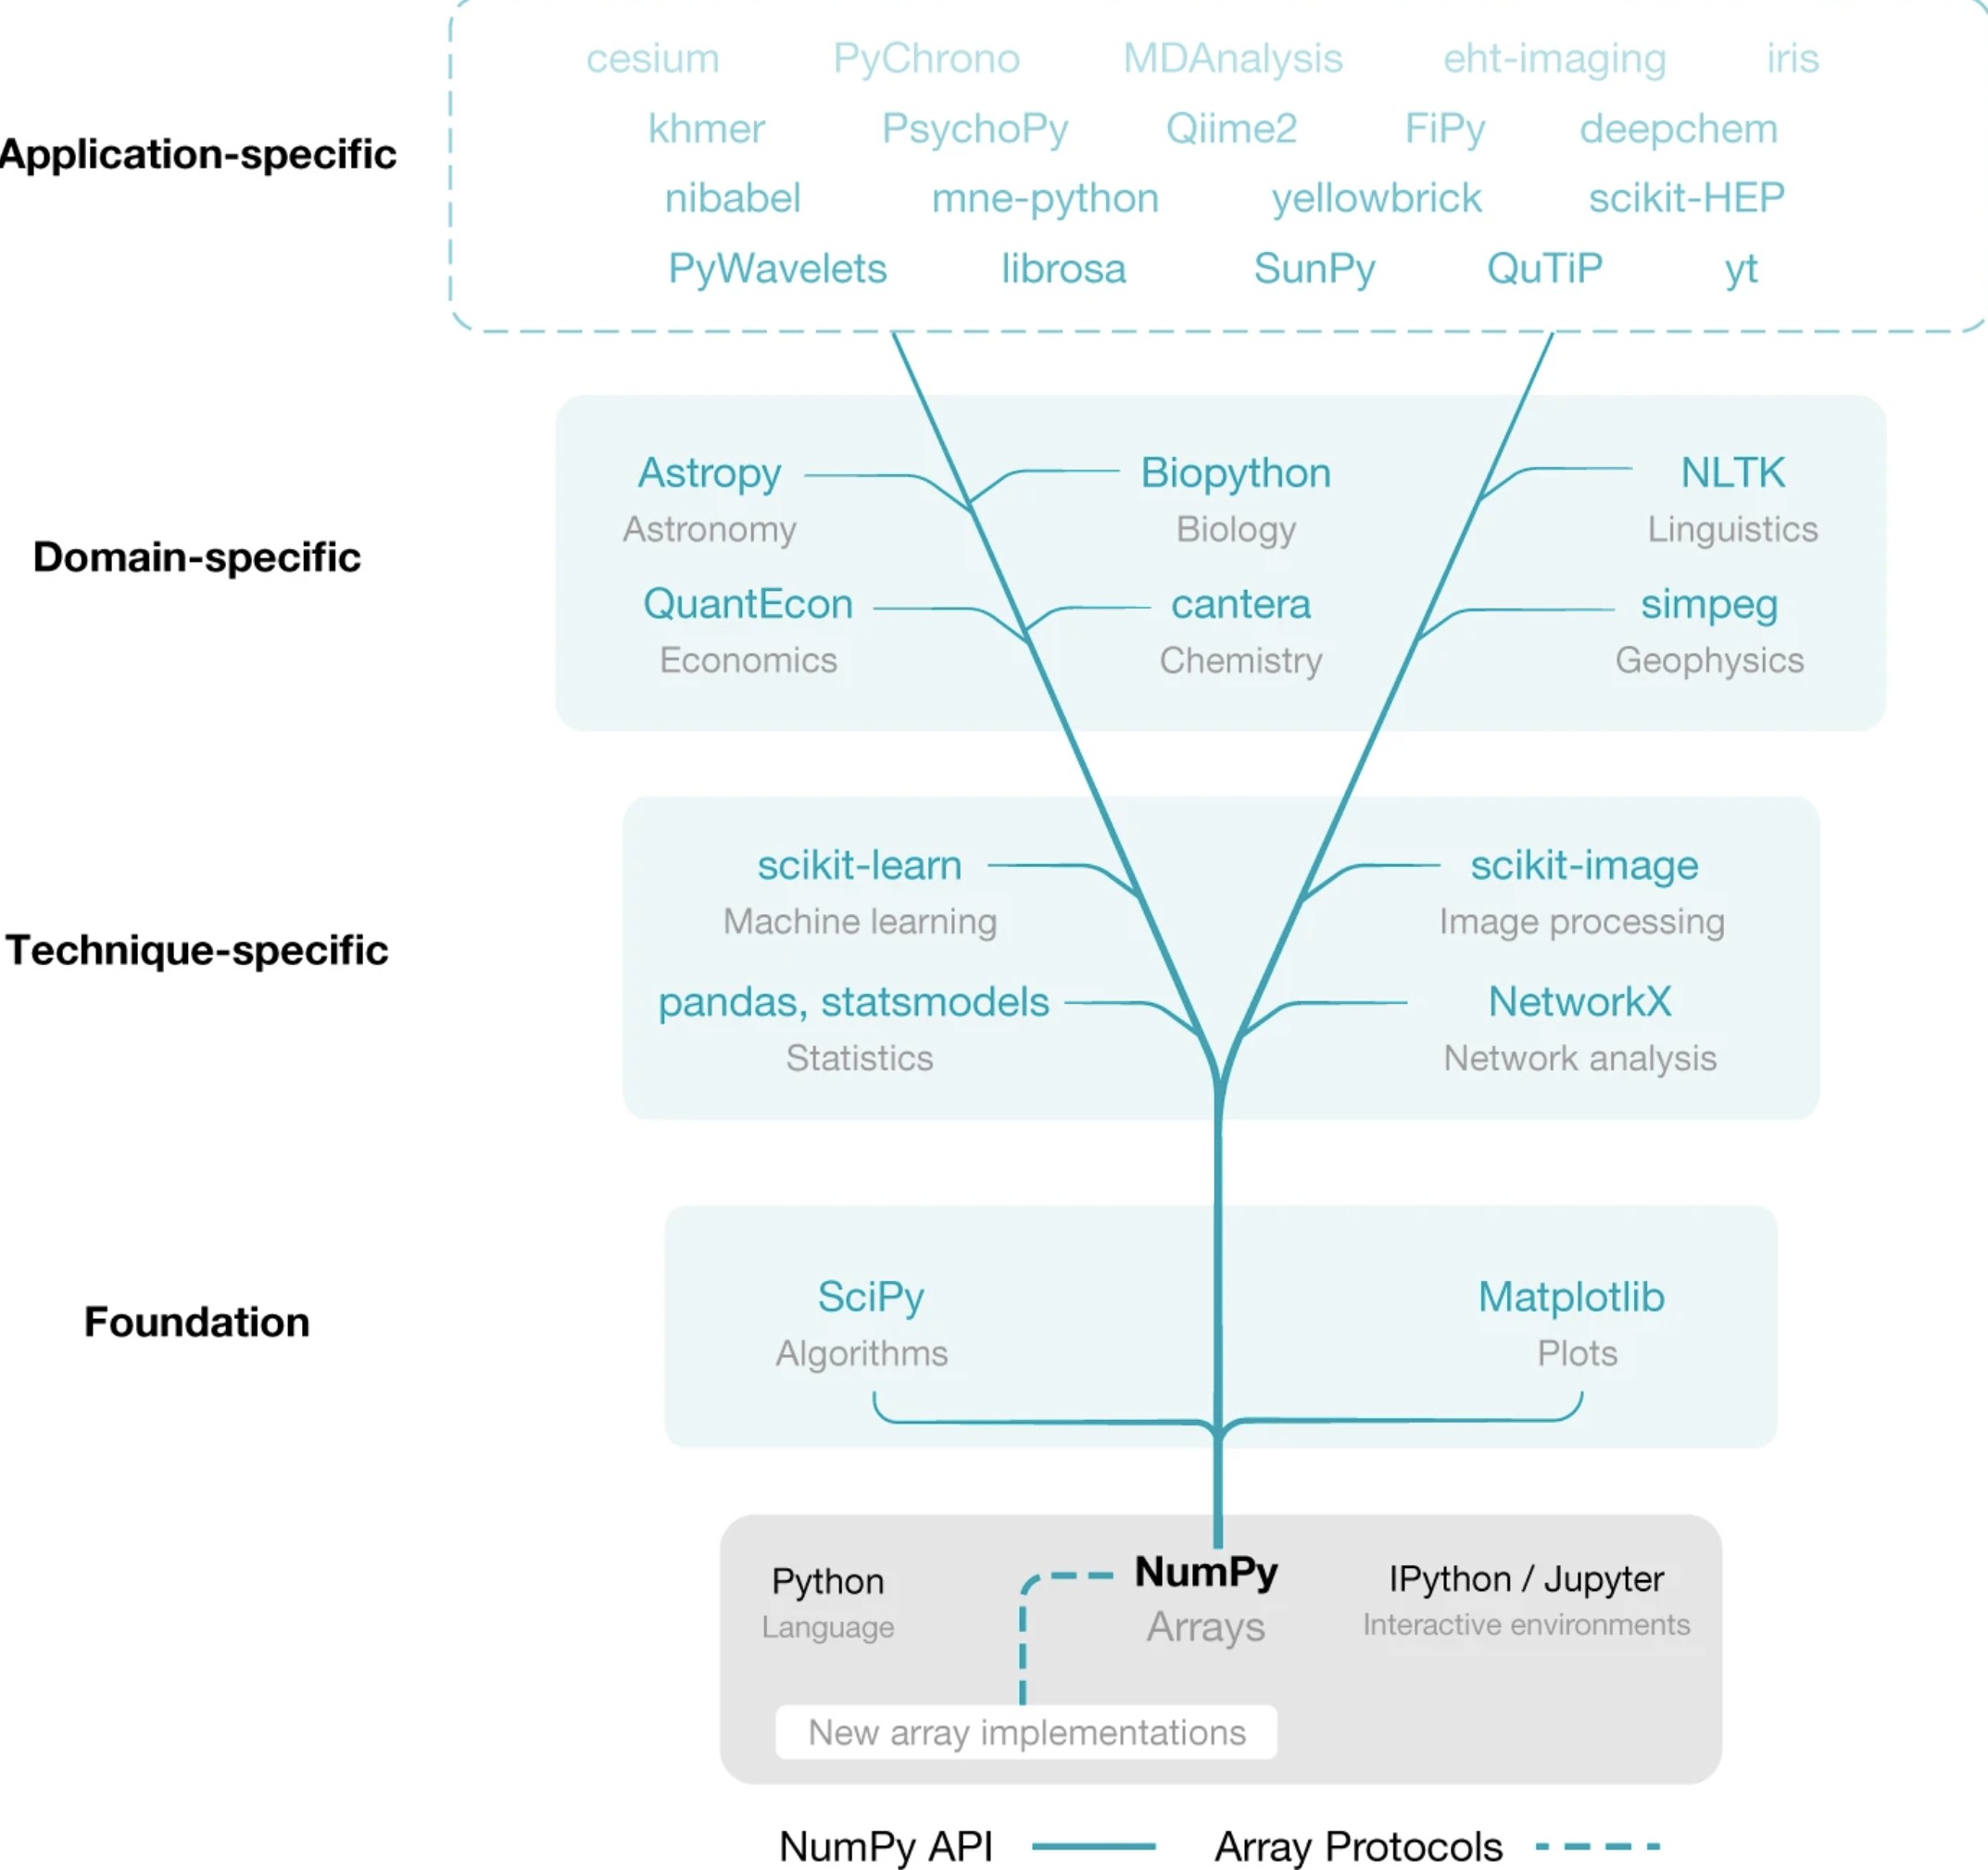
\includegraphics[width=\textwidth]{numpy_related_packs.png}}
\caption{گراف وابستگی کتاب‌خانه‌های پایتون به \lr{NumPy}\cite{van2011numpy}}
\label{fig:numpy_related_packs}
\end{figure}

\subsection{کتاب‌خانه‌ی \lr{Scikit-Learn}} 
\lr{Scikit-Learn}، جامع‌ترین و بزرگ‌ترین بسته یادگیری ماشین منبع‌باز در پایتون است. چون یادگیری ماشین اغلب به عنوان یک جزء از یک برنامه عمومی‌تر (همانند پروژه‌ی کنونی که به عنوان یک سرویس در وب توسعه داده‌شده است) استفاده می‌شود، ایده‌آل است که از همان زبان برنامه‌نویسی استفاده شود تا به‌صورت یکپارچه با سایر بخش‌های برنامه هماهنگ شود. با استفاده از قابلیت‌های گسترده پایتون، \lr{Scikit-Learn} به عنوان یک بسته محبوب برای برنامه‌های مرتبط با یادگیری ماشین در حال رشد است\cite{hao2019machine}. این کتاب‌خانه شامل توابع و اشیاء فراوانی برای مسائل طبقه‌بندی، رگرسیون، تقریب ماتریس کوواریانس، کاهش بعد و پیش‌پردازش داده‌ی خام می‌باشد\cite{kramer2016scikit}. اگرچه پایتون یک زبان برنامه‌نویسی تفسیری است، اما بیشتر روش‌های یادگیری ماشین در \lr{Scikit-Learn} بر پایه کتابخانه‌های دودویی کامپایل شده است که در ابتدا با زبان‌های فورتران\LTRfootnote{Fortran}، سی یا سی‌پلاس‌پلاس\LTRfootnote{C++} برنامه‌نویسی شده‌اند. این پیاده‌سازی‌های مبتنی بر دودویی‌ها به طور قابل توجهی کارایی محاسبات را بهبود می‌بخشند\cite{hao2019machine, kramer2016scikit}.

\section{جمع‌بندی و نتیجه‌گیری}
در این بخش، به تکنولوژی‌ها و چارچوب‌های اصلی استفاده‌شده برای توسعه‌ی مدل یادگیری ماشین اشاره کردیم. همانطور که در طول فصل بدان اشاره شد، زبان پایتون بدلیل دارا بودن غنی‌ترین کتابخانه‌های مربوط به محاسبات و یادگیری ماشین منطقی‌ترین انتخاب ممکن برای برگزیدن زبان توسعه‌ی مدل و سرویس هوش‌مصنوعی بود. دارا بودن چارچوب‌های با کارایی بالا برای توسعه برنامه‌ی وب نیز دیگر دلیل مهم برای انتخاب پایتون است.  ~
را در فایل 
\verb~AUTthesis.tex~،
غیرفعال%
\RTLfootnote{
برای غیرفعال کردن یک دستور، کافی است پشت آن، یک علامت
\%
 بگذارید.
}
 کنید. زیرا در غیر این صورت، ابتدا مطالب فصل ۱ و ۲ پردازش شده (که به درد ما نمی‌خورد؛ چون ما می‌خواهیم خروجی فصل ۳ را ببینیم) و سپس مطالب فصل ۳ پردازش می‌شود و این کار باعث طولانی شدن زمان اجرا می‌شود. زیرا هر چقدر حجم فایل اجرا شده، بیشتر باشد، زمان بیشتری هم برای اجرای آن، صرف می‌شود.

\subsection{مراجع}
برای وارد کردن مراجع به فصل 2
مراجعه کنید.
\subsection{واژه‌نامه فارسی به انگلیسی و برعکس}
برای وارد کردن واژه‌نامه فارسی به انگلیسی و برعکس، بهتر است مانند روش بکار رفته در فایل‌های 
\verb;dicfa2en;
و
\verb;dicen2fa;
عمل کنید.

\section{اگر سوالی داشتم، از کی بپرسم؟}
برای پرسیدن سوال‌های خود در مورد حروف‌چینی با زی‌پرشین،  می‌توانید به
 \href{http://forum.parsilatex.com}{تالار گفتگوی پارسی‌لاتک}%
\LTRfootnote{\url{http://www.forum.parsilatex.com}}
مراجعه کنید. شما هم می‌توانید روزی به سوال‌های دیگران در این تالار، جواب بدهید.
